\section{Infrared Thermography}

Infrared tomography is an imaging technique that utilizes infrared radiation emitted from nearly any objects. 
The existence of infrared radiation was first discovered in 1800 by Sir Frederick William Herschel. 
His experiments lead to the knowledge that there were a light spectrum beyond the visual spectrum humans are able to perceive.\cite{ignacio2017,optris2009}

Infrared thermography is commonly used to calculate surface temperatures and important concepts in the understanding of this are heat and temperature. 
Temperature is a measure for the internal energy within an object and can be defined as the average kinetic energy of the object.
Heat is the energy that passes from a warm object to another colder object. A warm object will decrease in internal energy and a cold object will increase due to the temperature difference and therefore the heat transfer. In the human body, a constant temperature is keep, due to several factors and therefore the temperature will not decrease even though a heat transfer to the surrounding environment occurs. The environmental temperature do have an impact on how large the heat transfer gradient is. If a body is in a cold environment, the emitted heat will be greater than the absorbed. In the same way, if the environment is much warmer than 37$^{\circ}$C, a greater absorption than emission will occur and the body will increase in temperature.\cite{ignacio2017} 



\subsection{Physical principals}

Any object above absolute zero emits energy-electromagnetic radiation depending on its temperature. Absolute zero is $0K$ or $ -273.16^{\circ}$C. To put that into perspective the human body has a temperature around 37$^{\circ}$C.\cite{ignacio2017,optris2009}

Electromagnetic radiation is a propagation of energy trough a medium without the transportation of mass. An electromagnetic wave is made of the relationship between frequency $f$, wavelength $\lambda$ and the speed of light $c$. This is stated in the equation of wave motion.\cite{ignacio2017}  
\begin{flalign}
	\lambda = \frac{c}{f}
	\label{eq:wave}
\end{flalign}
Depending on the frequency and wavelength certain characteristics arise from what is called the electromagnetic spectrum. The electromagnetic spectrum is the electromagnetic energy that is emitted. This extends from radiation of low energy such as radio waves and infrared, to waves of higher energy in form of eg. X-rays. A graphical representation of the electromagnetic spectrum can be seen on \cref{fig:em_spectrum}.\cite{ignacio2017}        

\begin{figure}[H]                                         
	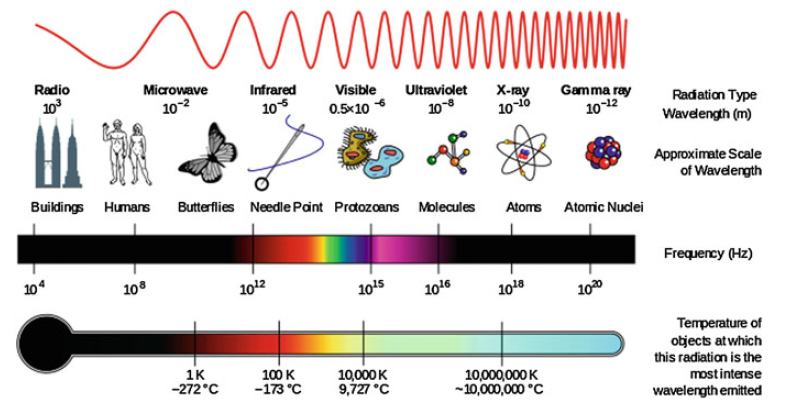
\includegraphics[width=.66\textwidth]{figures/em_spectrum}  
	\caption{The electromagnetic spectrum with wavelength, emitters, frequency and temperature.\cite{ignacio2017}}
	\label{fig:em_spectrum}  
\end{figure}   

Infrared radiation is also known as thermal radiation because of the relationship between temperature and infrared radiation. Temperature of the human body permits radiation in the infrared spectrum, but objects of much higher temperature are capable of emitting radiation in the visible and UV spectrum. This has to do with the difference between object and environmental temperature. If the temperature of these are relatively close to each other, the radiation emitted will be within infrared wavelengths. Infrared radiation has a wavelength from 769 nm to 1 mm. Objects emit more radiation in some region regions compared to others. Because of this is the infrared spectrum classified in the three regions, near, middle and far infrared. Near is between 769 nm and 2.5 $\mu$m, middle 2.5 $\mu$m to 50 $\mu$m and far 50 $\mu$m to 1 mm. The human body emits most radiation in the far infrared part, and most thermal cameras are build with this in mind. Near and middle cameras are used to measure gases.\cite{ignacio2017} 


\subsection{Measuring thermal energy}

The theory of the black body is important to understand the absorption and emission of light relative to temperature, because the theory of the black body is used to describe the laws of infrared radiation and its relationship to temperature. The black body is an ideal perfect emitter of infrared radiation because it absorbs all electromagnetic radiation permitted to it, and it emits the same amount of radiation as it absorbs, the absorption and emission sums up to be zero. 
Spectral emissive power, also denoted $E_\lambda$ is the energy emitted by a surface in relation to time and range of wavelength. Figure \ref{fig:Spectral} shows an graphical illustration of spectral emissive power of the black body for specific wavelengths when the temperature changes. Radiation at different frequencies according to temperature are also shown in the figure.\cite{ignacio2017} 

\begin{figure}[H]
	\centering	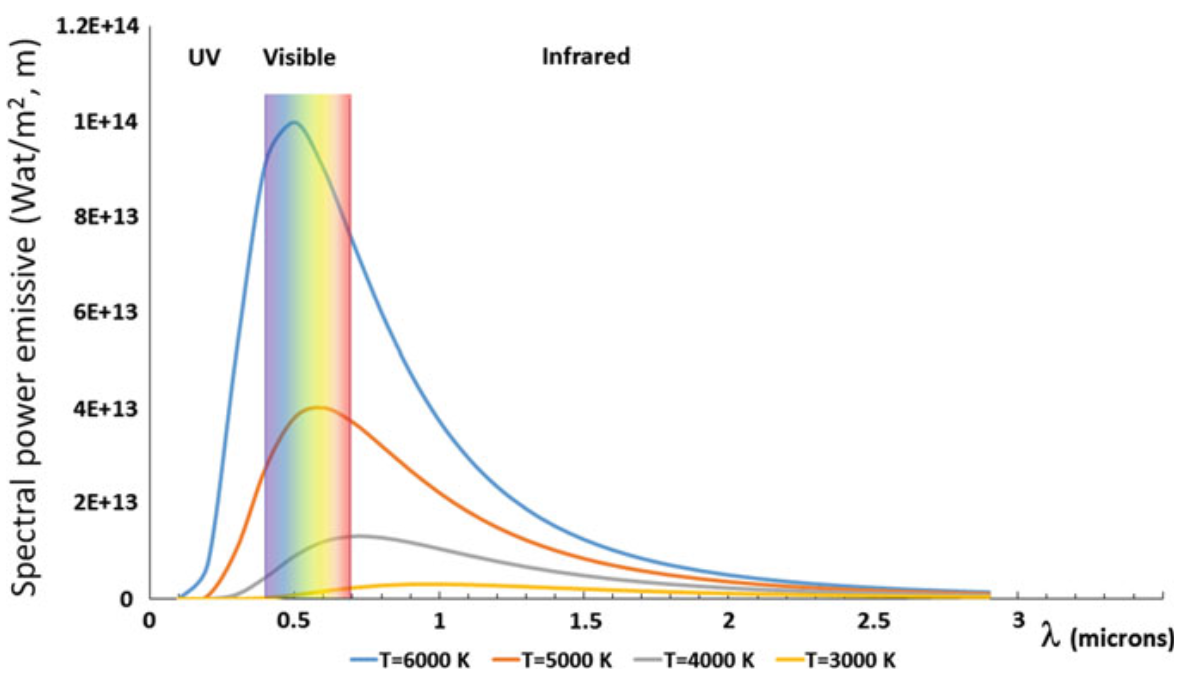
\includegraphics[width=0.65\textwidth]{figures/Spectral_power_emissive}
	\caption{Spectral power emissive\cite{ignacio2017}}
	\label{fig:Spectral}
\end{figure} \vspace{-.3cm}

The knowledge of this principle helps in the understanding of how infrared radiation behaves, and how temperature affects the frequency of the signal. 
The radiation from the human body which has a temperature at 37$^{\circ}$C emits the maximum energy of $9.3 \mu$m, which means that most of the radiation is in the far infrared spectrum.

- Maybe describe wien's displacement law... (wavelength of the peak of the blackbody radiation curve decreases as the body temperature increases)

- RIO (region of interest)
The lens are important to capture the image you want (dunno if this is relevant to mention?)



Measuring thermal radiation uses the knowledge that electromagnetic radiation is proportional to the internal energy. With a lens, the radiation that is emitted is focused onto a detector element in the camera that generates an electric output proportional to the radiation. The electric output is undergoing amplification and further signal processing.This allows the final output signal to be viewed as a temperature for the object. \cite{optris2009}
The black body is used for calibrating thermometers...

\begin{figure}[H]                                         
	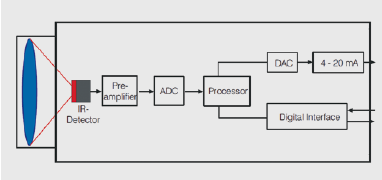
\includegraphics[width=.55\textwidth]{figures/IR_cam}  
	\caption{Simplified block diagram of an standard infrared camera.\cite{optris2009}}
	\label{fig:em_spectrum}  
\end{figure} 




%A bit more needs to be written here i think..
%
%
%Extra notes that i'we just copied that we can use later 
%
%The advantages of non-contact temperature measurement
%are obvious – it supports:
%
%• Temperature measurements of moving or overheated
%objects and of objects in hazardous surroundings
%
%• Very fast response and exposure times
%
%• Non-interactive measurement, no influence on
%the measuring object
%
%• Non-destructive measurement
%
%• Measurement point durability, no mechanical wear




